    \documentclass[12pt,a4paper]{article}
    \usepackage[utf8]{inputenc}
    \usepackage[T1]{fontenc}
    \usepackage[spanish]{babel}
    \usepackage{geometry}
    \geometry{margin=2.5cm}
    \usepackage{graphicx}
    \usepackage{booktabs}
    \usepackage{array}
    \usepackage{longtable}
    \usepackage{hyperref}
    \usepackage{xcolor}
    \usepackage{enumitem}
    \usepackage{fancyhdr}
    \usepackage{float}
    \usepackage{caption}
    \usepackage{multirow}
    
    \hypersetup{
        colorlinks=true,
        linkcolor=blue,
        urlcolor=blue,
        citecolor=blue
    }
    
    \pagestyle{fancy}
    \fancyhf{}
    \fancyhead[L]{\small ISR-401 -- Prueba Práctica Unidad IV}
    \fancyhead[R]{\small Sistema de Gestión de Pedidos}
    \fancyfoot[C]{\thepage}
    \renewcommand{\headrulewidth}{0.4pt}
    
    \begin{document}
    
    % ============================================
    % PORTADA
    % ============================================
    \begin{titlepage}
        \centering
        \vspace*{1cm}
        {\Large \textbf{Universidad Técnica Estatal de Quevedo}}\\[0.3cm]
        {\large Facultad de Ciencias de la Ingeniería}\\[0.3cm]
        {\large Carrera de Ingeniería de Software}\\[2cm]
    
        {\Huge \textbf{Prueba Práctica -- Unidad IV}}\\[0.5cm]
        {\LARGE Ingeniería de Requisitos (ISR-401)}\\[1.5cm]
    
        {\Large \textbf{Caso:} Sistema de Gestión de Pedidos}\\[2cm]
    
        \begin{tabular}{rl}
            \textbf{Docente:} & Ing. Gleiston Cicerón Guerrero Ulloa, PhD \\[0.2cm]
            \textbf{Estudiante:} & Mesías Quijije Jhon Alexander \\[0.2cm]
            \textbf{Asignatura:} & Ingeniería de Requisitos -- ISR-401 \\[0.5cm]
        \end{tabular}
    
            \vfill

\begin{figure}[H]
    \centering
    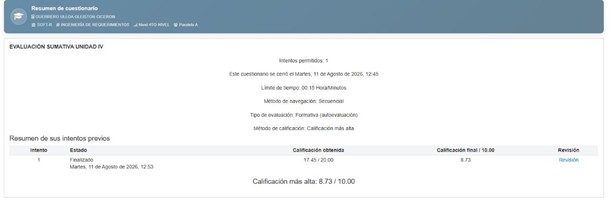
\includegraphics[width=0.55\textwidth]{diagrams/evidenciasga/evidenciasga1.jpg}
\end{figure}

\begin{figure}[H]
    \centering
    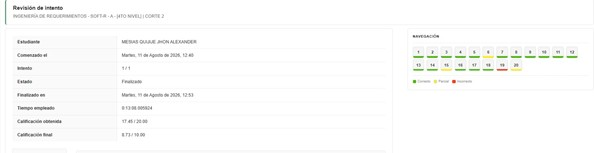
\includegraphics[width=0.55\textwidth]{diagrams/evidenciasga/evidenciasga2.jpg}
\end{figure}

    \vspace{0.5cm}
    {\large \textbf{Repositorio GitHub:}}\\[0.2cm]
    \url{https://github.com/jhonaelx24/Evaluacion-Practica-de-la-Unidad-IV}\\[0.8cm]

  {\large 11 de agosto de 2026}
\end{titlepage}

    % ============================================
    % ÍNDICE
    % ============================================
    \tableofcontents
    \newpage
    
    % ============================================
    % 1. CASO PRÁCTICO
    % ============================================
    \section{Caso práctico}
    
    \textbf{Sistema de Gestión de Pedidos} de una tienda en línea: un Cliente realiza cero o más Pedidos; cada Pedido contiene una o más Líneas de pedido, cada una referenciando un Producto. Al registrar un pedido se verifica el stock: si hay existencias se confirma, si no se notifica el faltante. Un pedido confirmado puede despacharse, luego entregarse, o anularse mientras no haya sido entregado.
    
    % ============================================
    % 2. P1. MODELO DE DATOS
    % ============================================
    \section{P1. Modelo de datos -- Diagrama de clases UML}
    
    \begin{figure}[H]
        \centering
        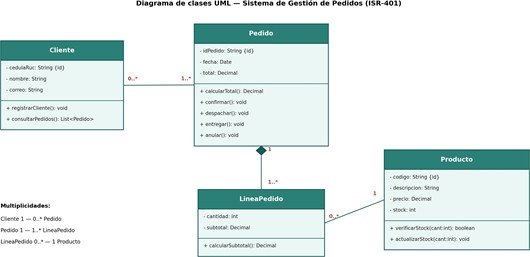
\includegraphics[width=0.95\textwidth]{diagrams/class_diagram}
        \caption{Diagrama de clases del dominio Sistema de Gestión de Pedidos}
        \label{fig:class}
    \end{figure}
    
    Los identificadores marcados con \texttt{\{id\}} son \texttt{Cliente.cedulaRuc}, \texttt{Pedido.idPedido} y \texttt{Producto.codigo}. \texttt{LineaPedido} se identifica por su posición dentro del Pedido, reforzada por la relación de composición (rombo relleno) entre Pedido y LineaPedido: una línea no existe sin su pedido y se elimina junto con él.
    
    Las multiplicidades correctas del dominio son:
    \begin{itemize}[nosep]
        \item \textbf{Cliente 1 -- 0..* Pedido:} un cliente puede tener cero o más pedidos.
        \item \textbf{Pedido 1 -- 1..* LineaPedido:} un pedido debe tener al menos una línea.
        \item \textbf{LineaPedido 0..* -- 1 Producto:} cada línea referencia exactamente un producto, y un producto puede aparecer en cero o más líneas.
    \end{itemize}
    
    \textbf{Nota de corrección:} En la imagen del diagrama de clases (Figura~\ref{fig:class}), las multiplicidades dibujadas en la asociación Cliente--Pedido aparecen invertidas respecto a la regla de negocio. La representación correcta es \textbf{1} junto a Cliente y \textbf{0..*} junto a Pedido.
    
    % ============================================
    % 3. P2. MODELO FUNCIONAL
    % ============================================
    \section{P2. Modelo funcional -- Diagrama de actividades UML}
    
    \begin{figure}[H]
        \centering
        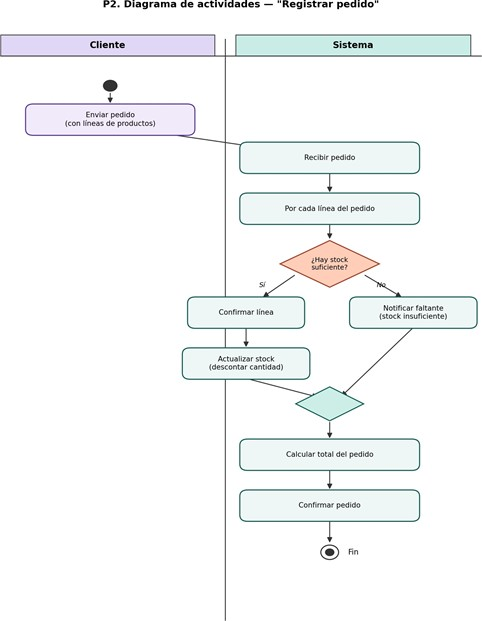
\includegraphics[width=0.85\textwidth]{diagrams/activity_diagram}
        \caption{Diagrama de actividades del proceso ``Registrar pedido'', con carriles Cliente / Sistema}
        \label{fig:activity}
    \end{figure}
    
    El proceso inicia en el carril Cliente con el nodo inicial, seguido de la acción ``Enviar pedido (con líneas de productos)'', que cruza al carril Sistema. Allí el flujo recibe el pedido y procesa cada línea (``Por cada línea del pedido'') hasta llegar al nodo de decisión ``¿Hay stock suficiente?''. La rama Sí confirma la línea y actualiza el stock del producto (descuenta la cantidad); la rama No notifica el faltante. Ambos caminos convergen en un nodo de unión antes de ``Calcular total del pedido'' y ``Confirmar pedido'', cerrando en el nodo final del carril Sistema.
    
    % ============================================
    % 4. P3. MODELO DE COMPORTAMIENTO
    % ============================================
    \section{P3. Modelo de comportamiento -- Máquina de estados UML}
    
    \begin{figure}[H]
        \centering
        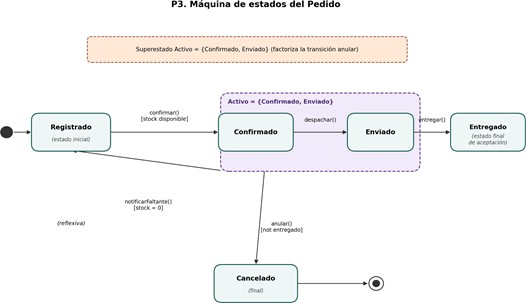
\includegraphics[width=0.95\textwidth]{diagrams/state_machine}
        \caption{Máquina de estados del ciclo de vida de un Pedido}
        \label{fig:state}
    \end{figure}
    
    El superestado \textit{Activo} agrupa los estados \textit{Confirmado} y \textit{Enviado}, factorizando en una sola transición de salida el evento \texttt{anular()[not entregado]} hacia \textit{Cancelado} (estado final). El estado \textit{Registrado} es el estado inicial y tiene una transición reflexiva \texttt{notificarFaltante()[stock = 0]} que lo mantiene en Registrado cuando la verificación de stock falla. El evento \texttt{confirmar()[stock disponible]} lleva de Registrado a Confirmado; \texttt{despachar()} lleva a Enviado; \texttt{entregar()} lleva a Entregado, marcado como estado final de aceptación.
    
    % ============================================
    % 5. P4. CONSISTENCIA
    % ============================================
    \section{P4. Consistencia entre las tres perspectivas}
    
    \subsection*{Tabla de verificación cruzada}
    
    \begin{table}[H]
    \centering
    \begin{tabular}{@{}p{4.2cm}p{4.5cm}p{5.5cm}@{}}
    \toprule
    \textbf{Evento (P3)} & \textbf{Función/acción (P2)} & \textbf{Entidad/atributo (P1) modificado} \\
    \midrule
    \texttt{confirmar()} [stock disponible] & Confirmar línea $\rightarrow$ Actualizar stock (rama Sí) & \texttt{Producto.stock} vía \texttt{actualizarStock(cant)}; estado del Pedido \\
    \texttt{notificarFaltante()} [stock = 0] & Notificar faltante (stock insuficiente) (rama No) & Sin modificación de atributos; notificación al cliente \\
    \texttt{despachar()} & (Sin acción explícita en P2; P2 modela solo Registrar pedido) & \texttt{Pedido.despachar()} \\
    \texttt{entregar()} & (Sin acción explícita en P2) & \texttt{Pedido.entregar()} \\
    \texttt{anular()} [not entregado] & (Sin acción explícita en P2) & \texttt{Pedido.anular()} \\
    \bottomrule
    \end{tabular}
    \end{table}
    
    \subsection*{Inconsistencias detectadas y correcciones}
    
    \begin{enumerate}[label=\textbf{Defecto \arabic*:}]
        \item \textbf{(P1, asociación Cliente--Pedido):} En el diagrama de clases, las multiplicidades dibujadas junto a la línea de asociación son \texttt{0..*} en el extremo de Cliente y \texttt{1..*} en el extremo de Pedido. Esto contradice tanto la leyenda del propio diagrama (Cliente 1 -- 0..* Pedido) como la regla de negocio del caso (un Cliente puede realizar cero o más Pedidos): con la lectura dibujada, un Pedido quedaría asociado a 0..* Clientes (un pedido sin dueño claro) y cada Cliente exigiría 1..* Pedidos (ningún cliente podría tener cero pedidos), lo que rompe el enunciado del caso práctico.
    
        \textbf{Corrección aplicada:} Se invierten las multiplicidades del extremo de la asociación Cliente--Pedido para que queden \textbf{1} junto a Cliente y \textbf{0..*} junto a Pedido, alineando el diagrama con su propia leyenda y con la regla de negocio del caso.
    
        \item \textbf{(P1 vs. P3):} El evento \texttt{notificarFaltante()} (transición reflexiva sobre Registrado en P3, y acción ``Notificar faltante'' en P2) no tiene una operación equivalente en ninguna clase de P1. Pedido solo declara \texttt{calcularTotal()}, \texttt{confirmar()}, \texttt{despachar()}, \texttt{entregar()} y \texttt{anular()}.
    
        \textbf{Corrección aplicada:} Se añade \texttt{+ notificarFaltante(): void} a la clase Pedido para cerrar la trazabilidad funcional entre las tres perspectivas.
    \end{enumerate}
    
    % ============================================
    % 6. P5. ESPECIFICACIÓN DE REQUISITOS
    % ============================================
    \section{P5. Especificación de requisitos con esquema de atributos}
    
    \begin{itemize}[leftmargin=*]
        \item \textbf{RF-01:} El sistema debe registrar un nuevo pedido validando la disponibilidad de stock de cada producto solicitado.
        \item \textbf{RF-02:} El sistema debe permitir anular un pedido siempre que no haya sido entregado.
        \item \textbf{RNF-01 (Eficiencia de desempeño -- ISO/IEC 25010):} El sistema debe confirmar o rechazar el registro de un pedido en menos de 3 segundos bajo carga normal ($\leq$ 50 pedidos concurrentes).
        \item \textbf{RNF-02 (Seguridad -- ISO/IEC 25010):} Los datos personales del cliente (cédula/RUC, correo) deben almacenarse cifrados en reposo (AES-256) y transmitirse únicamente mediante TLS 1.2 o superior.
    \end{itemize}
    
    \begin{table}[H]
    \centering
    \small
    \begin{tabular}{@{}p{1.3cm}p{1.3cm}p{1.5cm}p{2.8cm}p{1.5cm}p{1cm}p{3.5cm}@{}}
    \toprule
    \textbf{ID} & \textbf{Prioridad} & \textbf{Estado} & \textbf{Fuente} & \textbf{Estabilidad} & \textbf{Ver.} & \textbf{Método de verificación} \\
    \midrule
    RF-01 & Alta & Propuesto & Caso de estudio, \S2 (regla de stock) & Estable & 1.0 & Prueba funcional (CP-01) \\
    RF-02 & Alta & Propuesto & Caso de estudio, \S2 (ciclo de vida del pedido) & Estable & 1.0 & Prueba funcional (CP-02) \\
    RNF-01 & Media & Propuesto & Requisito de negocio (experiencia de usuario) & Media & 1.0 & Prueba de rendimiento/carga (CP-03) \\
    RNF-02 & Alta & Propuesto & Política de protección de datos personales & Estable & 1.0 & Prueba de seguridad/auditoría de cifrado (CP-04) \\
    \bottomrule
    \end{tabular}
    \caption{Esquema de atributos de requisitos}
    \end{table}
    
    % ============================================
    % 7. P6. PRIORIZACIÓN MoSCoW
    % ============================================
    \section{P6. Priorización MoSCoW}
    
    \begin{itemize}[leftmargin=*]
        \item \textbf{RF-01 -- Must have.} Es la funcionalidad núcleo del dominio: sin verificación y registro de pedidos el sistema no cumple su propósito.
        \item \textbf{RNF-02 -- Must have.} La protección de datos personales es una obligación explícita del caso (proteger los datos personales del cliente) y de cumplimiento normativo; omitirla implica riesgo legal y de reputación.
        \item \textbf{RF-02 -- Should have.} Importante para completar el ciclo de vida del pedido, pero el sistema puede operar en un primer incremento sin anulación automatizada (proceso manual transitorio).
        \item \textbf{RNF-01 -- Could have.} Deseable para una buena experiencia de usuario, pero no bloquea la operación básica del sistema si se entrega en una iteración posterior.
    \end{itemize}
    
    % ============================================
    % 8. P7. VALIDACIÓN POR INSPECCIÓN
    % ============================================
    \section{P7. Validación por inspección (checklist ISO/IEC/IEEE 29148)}
    
    \subsection*{Paso 1 -- Identificación de defectos (sin corregir)}
    
    Propiedades evaluadas: no ambiguo, completo, singular, verificable, factible.
    
    \begin{table}[H]
    \centering
    \small
    \begin{tabular}{@{}clp{3.5cm}p{6.5cm}@{}}
    \toprule
    \textbf{ID} & \textbf{Requisito} & \textbf{Propiedad violada} & \textbf{Descripción del defecto} \\
    \midrule
    D-01 & RF-01 & Completo & No define el comportamiento cuando solo una parte de los productos del pedido tiene stock disponible. \\
    D-02 & RF-02 & No ambiguo & No especifica qué rol/actor está autorizado para anular el pedido. \\
    D-03 & RNF-01 & Verificable & No define el entorno/condiciones de medición (hardware, red) necesarias para reproducir la métrica de 3 s. \\
    D-04 & RNF-02 & Singular & Combina dos mecanismos de seguridad distintos (cifrado en reposo y cifrado en tránsito) en un mismo enunciado. \\
    \bottomrule
    \end{tabular}
    \caption{Defectos identificados en la inspección}
    \end{table}
    
    \subsection*{Paso 2 -- Retrabajo (requisitos corregidos)}
    
    \begin{itemize}[leftmargin=*]
        \item \textbf{RF-01 (v1.1):} El sistema debe registrar un pedido solo si todos los productos solicitados tienen stock suficiente; si algún producto no tiene stock suficiente, el sistema debe rechazar el registro e indicar el/los producto(s) que generaron el faltante.
        \item \textbf{RF-02 (v1.1):} El sistema debe permitir que el Cliente propietario del pedido o un Administrador anulen un pedido, siempre que su estado no sea Entregado.
        \item \textbf{RNF-01 (v1.1):} En un entorno de referencia (servidor de 4 vCPU / 8 GB RAM, red interna $\leq$ 5 ms de latencia) y bajo carga normal ($\leq$ 50 pedidos concurrentes), el sistema debe confirmar o rechazar el registro de un pedido en menos de 3 segundos en el 95\% de las solicitudes.
        \item \textbf{RNF-02a (v1.1):} Los datos personales del cliente (cédula/RUC, correo) deben almacenarse cifrados en reposo utilizando AES-256.
        \item \textbf{RNF-02b (v1.1):} Toda comunicación cliente-sistema que transmita datos personales debe utilizar TLS 1.2 o superior.
    \end{itemize}
    
    % ============================================
    % 9. P8. PRUEBAS DE ACEPTACIÓN
    % ============================================
    \section{P8. Pruebas de aceptación trazadas}
    
    \begin{table}[H]
    \centering
    \small
    \begin{tabular}{@{}p{1.3cm}p{2cm}p{4.5cm}p{4.5cm}p{1.5cm}@{}}
    \toprule
    \textbf{ID} & \textbf{Tipo} & \textbf{Entradas} & \textbf{Criterio de éxito} & \textbf{Traza} \\
    \midrule
    CP-01 & Funcional & Pedido con producto A (stock = 5, solicita 2) y producto B (stock = 0, solicita 1) & El sistema rechaza el pedido completo e indica el código del producto B como causante del faltante & RF-01 \\
    \addlinespace
    CP-02 & Funcional & Pedido en estado Confirmado; solicitud de anulación por el cliente propietario. Caso negativo: solicitud sobre pedido Entregado & El pedido pasa a Cancelado con fecha/hora registrada; el caso negativo es rechazado & RF-02 \\
    \addlinespace
    CP-03 & No funcional & 50 solicitudes de registro concurrentes en entorno de referencia & El percentil 95 del tiempo de respuesta es menor a 3 s & RNF-01 \\
    \addlinespace
    CP-04 & No funcional (seguridad) / regresión & Cliente nuevo; inspección de base de datos durante el registro & La cédula/RUC y el correo aparecen cifrados en la base de datos (AES-256); el tráfico de red usa TLS 1.2+ & RNF-02 \\
    \bottomrule
    \end{tabular}
    \caption{Casos de prueba de aceptación}
    \end{table}
    
    % ============================================
    % 10. P9. MATRIZ DE TRAZABILIDAD
    % ============================================
    \section{P9. Matriz de trazabilidad}
    
    \begin{table}[H]
    \centering
    \small
    \begin{tabular}{@{}p{1.5cm}p{3.5cm}p{4.5cm}p{1.5cm}p{3.5cm}@{}}
    \toprule
    \textbf{Req.} & \textbf{Fuente (traza atrás)} & \textbf{Modelos (traza adelante)} & \textbf{Prueba} & \textbf{Observación} \\
    \midrule
    RF-01 & Caso de estudio \S2: el sistema verifica la disponibilidad de stock & P1: \texttt{Producto.stock}, \texttt{verificarStock()}, \texttt{actualizarStock()}; P2: ``¿Hay stock suficiente?'' / ``Actualizar stock''; P3: \texttt{confirmar()[stock disponible]}, \texttt{notificarFaltante()[stock = 0]} & CP-01 & --- \\
    \addlinespace
    RF-02 & Caso de estudio \S2: puede anularse mientras no haya sido entregado & P3: \texttt{anular()[not entregado]} (transición del superestado Activo); P1: \texttt{Pedido.anular()} & CP-02 & Depende de RF-01 (dependencia horizontal: no puede anularse un pedido que no ha sido registrado) \\
    \addlinespace
    RNF-01 & Requisito de rapidez & Sin modelo estructural explícito & CP-03 & Huérfano de modelo: las NFR de rendimiento no se representan en los diagramas UML estructurales; solo tienen traza a prueba. Se recomienda documentarlo como una nota de rendimiento asociada a las operaciones \texttt{Pedido.confirmar()} y \texttt{Pedido.calcularTotal()}. \\
    \addlinespace
    RNF-02 & Caso de estudio: datos personales del cliente & P1: \texttt{Cliente.correo}, \texttt{Cliente.cedulaRuc} & CP-04 & --- \\
    \bottomrule
    \end{tabular}
    \caption{Matriz de trazabilidad de requisitos}
    \end{table}
    
    \textbf{Dependencia horizontal:} RF-02 $\rightarrow$ RF-01 (un pedido debe existir/registrarse antes de poder anularse).
    
    % ============================================
    % 11. P10. GESTIÓN DEL CAMBIO
    % ============================================
    \section{P10. Gestión del cambio y línea base}
    
    \subsection*{Solicitud de cambio}
    
    \textbf{SC-01 -- Solicitante:} Jefe de Ventas.\\
    \textbf{Fecha:} 2026-08-11.\\
    \textbf{Requisito afectado:} RF-02 (v1.1).\\
    \textbf{Descripción:} Permitir que, además del Cliente propietario y el Administrador, un Supervisor de bodega pueda anular un pedido cuando detecte un error de picking antes del despacho.
    
    \subsection*{Análisis de impacto (usando la matriz de P9)}
    
    \begin{itemize}[leftmargin=*]
        \item Afecta directamente a RF-02 y a su prueba CP-02 (debe añadirse un caso con actor Supervisor de bodega).
        \item Por la dependencia horizontal RF-02 $\rightarrow$ RF-01, RF-01 no se ve impactado en su lógica de negocio.
        \item Si se decide registrar quién ejecuta la anulación, debe agregarse el atributo \texttt{Pedido.actorAnulacion: String} en P1 (impacto menor en el diagrama de clases). La máquina de estados (P3) no cambia: la guarda \texttt{[pedido no entregado]} sigue siendo válida para el nuevo actor.
    \end{itemize}
    
    \subsection*{Decisión del CCB}
    
    \textbf{Aprobada} (Comité de Control de Cambios, 2026-08-13), condicionada a: (1) agregar \texttt{Pedido.actorAnulacion} en P1, y (2) actualizar CP-02 con el nuevo caso de prueba para el Supervisor de bodega.
    
    \textbf{Nueva versión de RF-02:} El sistema debe permitir que el Cliente propietario del pedido, un Administrador o un Supervisor de bodega anulen un pedido, siempre que su estado no sea Entregado.
    
    \subsection*{Línea base}
    
    \begin{itemize}[leftmargin=*]
        \item \textbf{Baseline B1.0} (2026-08-11, antes del cambio): ERS v1.1 (requisitos reworked de P7), P1 v1.0, P2 v1.0, P3 v1.0, matriz de trazabilidad (P9) v1.0, pruebas de aceptación (P8) v1.0.
        \item \textbf{Baseline B1.1} (2026-08-13, tras aprobación de SC-01): RF-02 v1.2, P1 v1.1 (con \texttt{actorAnulacion}), CP-02 v1.1, matriz de trazabilidad v1.1; el resto de artefactos hereda sin cambios de B1.0.
    \end{itemize}
    
    \end{document}
